\documentclass[12pt]{article}
\usepackage{setspace}
\doublespacing


%% preamble: Keep it clean; only include those you need
\usepackage{amsmath}
\usepackage[margin = 1in]{geometry}
\usepackage{graphicx}
\usepackage{booktabs}
\usepackage{natbib}

% highlighting hyper links
\usepackage[colorlinks=true, citecolor=blue]{hyperref}


%% meta data
\title{Data analytics effects in Baseball player's value}
\author{Chenyu Mu\\
  Department of Statistics\\
  University of Connecticut
}

\begin{document}

\maketitle

\begin{abstract}
  Over the past two decades, there has been a notable resurgence in the utilization of data analytics across 
  professional sports, businesses, and governmental sectors. We can measure the value of baseball players through
  data analysis, which is very important to the success of the team. Therefore, this article will study how to 
  measure the value of a player and will delve into an in-depth analysis of the myriad factors that potentially 
  impact baseball players while they are actively engaged in the game. 
\end{abstract}


\section{Introduction}
\label{sec:intro}
  
The surge in the availability of data, from player statistics to in-game metrics, has ushered in a new era in 
baseball analysis. This wealth of information has not only enriched the fan experience but has also become an 
invaluable tool for teams and analysts seeking a competitive edge. So how do we measure the value of players in
a statistical way?Before discussing how to measure value, we need to discuss the definition of value. 
According to the definition in Wyers' article "How to measure a player's value"\cite*{web:Wyers:Part1}, we define 
the value of a player as "A player's value is his contributions to his team based upon his on-field performance 
(hitting, running, fielding and pitching) in a neutral context.This definition excludes qualities like leadership 
and character, which would be horrific to see a statistical measure of performance attempt to portray! That's not 
to argue these things don't matter; they just aren't easily quantified. In addition, according to Wyers' approach, 
we need to emphasize that this is a neutral environment. First, we want to quantify a player's performance apart 
from his teammates' - a player is no better or worse on a good or terrible team. Besides, we aim to separate a 
player from his surroundings. A terrible pitcher does not become a better pitcher by pitching in Petco Park, and 
a poor hitter does not become a better pitcher by hitting in Coors Field.\\

We should realize there are some limits may effects our statistical model:
\begin{enumerate}
\item The data itself. Errors can occur, including transcription errors and similar inaccuracies. Additionally, 
certain determinations rely on borderline judgments, such as discerning whether an event constitutes a hit or an
error, categorizing a hit as a fly ball or a line drive, and determining whether a pitch is a ball or a strike.

\item Critical information might be omitted from the data, necessitating inference or deliberate oversight. 
Questions such as the shortstop's positioning on the field or whether the coach executed a hit-and-run strategy may 
not be explicitly recorded and might require additional interpretation or intentional exclusion.

\item Developing a model without a grasp of the fundamental principles poses challenges. The inherent value
difference between a double and a sacrifice fly in baseball may be intuitive, but expressing and capturing this 
nuanced understanding can be particularly challenging for a linear regression model.

\item The model overlooks certain factors, such as the quality of the opponent, platoon advantage, and other 
relevant considerations.

\item Neglecting to consider subtle distinctions between players, such as the influence of a ballpark on the home 
run rates of individuals like Barry Bonds and Juan Pierre, can lead to oversights in the analysis.
\end{enumerate}

Every value indicator has an underlying baseline, whether by chance or design. As a result, it is advisable to 
carefully analyze the choice of a baseline and the reasoning behind it. Baselines are important since we are not 
interested in a single player - there is no such thing as a baseball player in isolation. We're interested in a 
player's contributions in the context of a team - the marginal contribution of that player in comparison to who 
else could have played instead. If you've ever spent a lot of time on baseball forums or message boards, you've 
probably seen an idea that starts with, "What could it hurt to do this?" It's the opportunity cost: playing time 
is a fixed commodity that cannot be transferred from one player to another. Now let's start to talk about the
detail process of value baseball players.


% roadmap
The rest of the paper is organized as follows.

The data will be presented in Section~\ref{sec:data}.

The methods are described in Section~\ref{sec:meth}.

The results are reported in Section~\ref{sec:resu}.

A discussion concludes in Section~\ref{sec:disc}.

\section{Data}
\label{sec:data}


We got the 2008 season stats for 30 teams from Fangraphs website, including team name, plate appearence, average, 
pitches and so on. We then process the data we collect using the code mentioned in Figure~ \ref*{fig:baseballcode}.The 
data \ref{tab:PF_PFPA} and all player data is drawn from the Stats section of Fangraphs \cite*{web:data}. 

\begin{figure}[tbp]
  \centering
  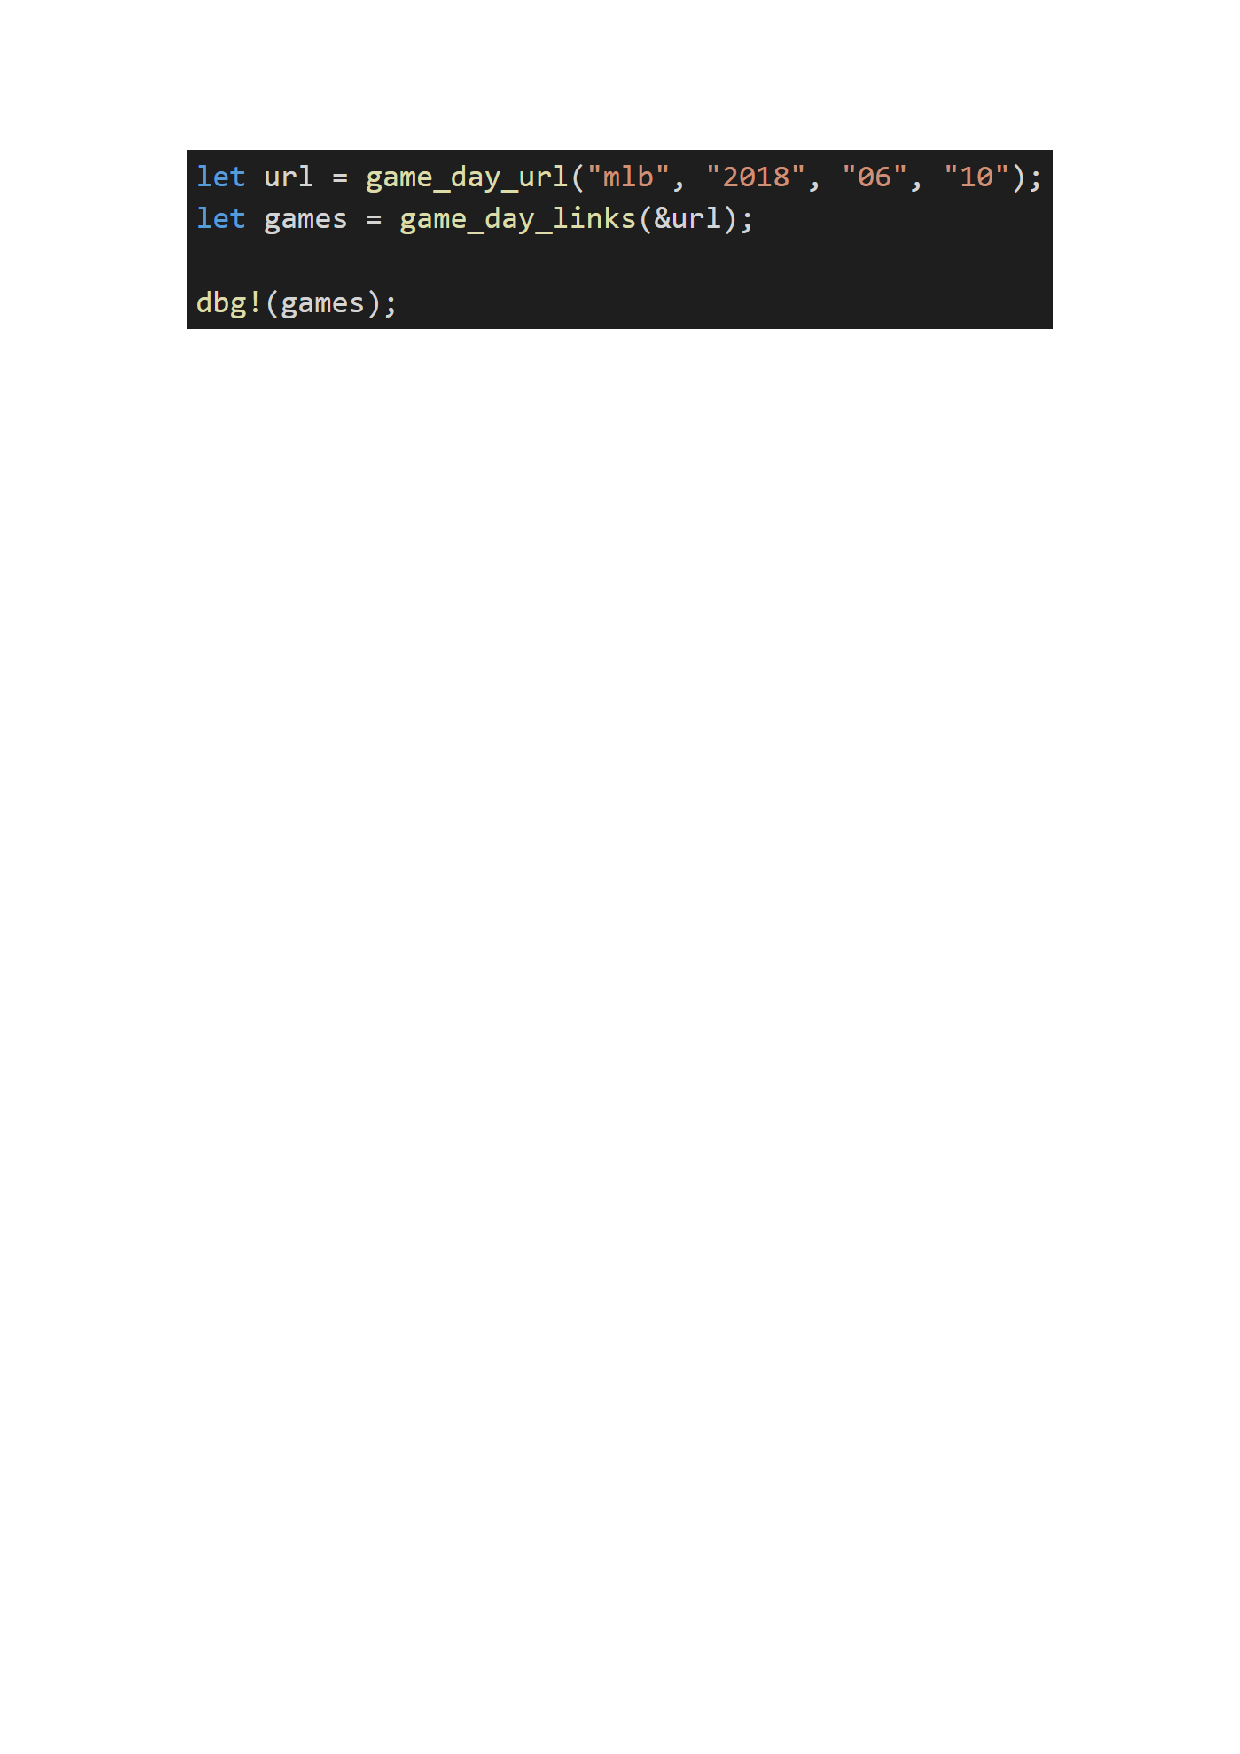
\includegraphics[width=\textwidth]{baseballcode.pdf}
  \caption{code for addressing stats 2008 baseball team}
  \label{fig:baseballcode}
\end{figure}



\section{Methods}
\label{sec:meth}

As Wyers mentioned  "A player's value is essentially an average team's 
runs or wins with that player, minus their runs or wins without that player." \citep*{web:Wyers:Part2} We have two 
types of models: dynamic and linear. Dynamic models excel in assessing entire contexts, such as a team's overall performance or 
a pitcher's effectiveness. However, they are less effective when applied to individual hitters, as each hitter 
only influences a fraction of the overall context. Additionally, a hitter's performance 
does not interact with itself; for instance, if a hitter walks, they cannot subsequently hit a home run to drive 
themselves in.

On the other hand, linear models are adept at capturing the environmental context, making them 
well-suited for estimating a hitter's contribution to a specific context. However, they may not perform as 
effectively when evaluating pitchers. 

Among dynamic run estimators, BaseRuns stands out as the most accurate and versatile. The formula for BaseRuns is:

\begin{equation}
  \label{eq:baseRuns}
A*B/(B + C) + D
\end{equation}

Where $A$ is the number of baserunners, $B$ is the “advancement factor,” $C$ is the number of outs, and $D$ is the 
number of home runs.

There are nearly too many linear weights formulas to name when it comes to linear run estimators. It's generally 
ideal to utilize bespoke linear weights dependent on the season for a player value system. The most important 
factor to consider is baseline—while all dynamic run estimators provide absolute runs, certain linear run estimators
provide runs above average instead. 

Measuring playing time in baseball isn't always straightforward. At the team level, the fundamental unit is the
out, crucial for both offense and defense. Pitchers and fielders often use outs, games, or innings, but when 
it comes to batting, plate appearances or at-bats are commonly used. The challenge arises as plate appearances 
are not fixed, impacting a player's contribution.Most run estimators focus on runs per out,
emphasizing the importance of using the correct unit of playing 
time. Linear run estimators typically use plate appearances. It's crucial to recognize that comparing players 
should consider the same number of batting outs, not plate appearances.To make it more relatable, 
some analysts convert runs per out to runs per plate appearance. This simplification 
helps those more accustomed to plate appearances as the unit of playing time for hitters. The key is precision 
when comparing and evaluating player performance metrics.

In sabermetrics, it's widely accepted that a player's runs contribution should be separated from the 
impact of their home park. The debate revolves around using either simple, run-based park factors or more 
detailed component park factors.

For a value metric, the general preference is for run-based park factors. This adjustment accounts 
for the fact that the value of a run can vary based on the ballpark - for instance, a run in Coors is 
considered less valuable than a run in Petco. While there are situations where component park factors might 
be relevant, they don't necessarily provide a "more accurate" assessment of a player's value, especially 
concerning explaining team wins. The choice between the two depends on the specific analysis goals and nuances.

Fielding value is more difficult to quantify because, while there is only one hitter, the defense has nine 
fielders on every play. It is quite simple to determine who made a specific play, but it is frequently 
difficult to determine who should be liable for a ball when no play is made. Various defensive metrics attempt 
to determine who is responsible for a ball in play. In general, the better the outcomes, the more detailed the 
underlying dataset.

Table~\ref*{tab:discription}are definitions we may use 
\begin{table}[htbp]
  \caption{Baseball Batting Statistics}
  \label{tab:discription} 
  \centering
  \begin{tabular}{|l|l|}
     \hline
     \textbf{Variable} & \textbf{Description}\\
     \hline
     $AB$ & At bats\\
     $AVG$ & Batting average\\
     $H$ & Hits\\
     $K$ & Strikeouts\\
     $HR$ & Home Run\\
     $BABIP$ & Batting Average on Balls in Play\\
     $SF$ & Sacrifice flies\\
    \hline
  \end{tabular}
\end{table}

\begin{equation}
  \label{eq:AVG}
  AVG = H/AB,
\end{equation}
which means the total number of hits divided by the total number of at-bats
\begin{equation}
  \label{eq:BABIP}
  BABIP = (H - HR) / (AB - K - HR - SF),
\end{equation}
which states that a batter's average for balls that are put in play (excludes strikeouts, home runs, and 
sacrifice flies)




\section{Results}
\label{sec:resu}
In assessing a player's offensive value, a linear system proves to be most effective. Linear systems
provide insights into the number of runs a player adds to an average team. It's important 
to note that linear weights values may not necessarily sum up to team totals accurately, 
particularly for teams that excel or struggle significantly on the offensive front. If we're going to use a 
linear run estimator, shouldn't we also use a linear park factor? We simply 
take the average number of runs per plate appearance—roughly.122 in 2008—and park compensate for the 
difference. Simply multiply that figure by the number of plate appearances and add it to the 
linear weight values to get your park adjustment. And that is all there is to it. Simply put, 
you have a measure of a player's offensive worth relative to the average.
This gives us a linear factor to work with, as shown Table~ \ref*{tab:PF_PFPA}

\begin{table}[ht]
  \caption{Park value formula and its per plate appearance in each team}
  \label{tab:PF_PFPA} 
  \centering
  \resizebox{\columnwidth}{!}{
    \begin{tabular}{|l|c|c|c|c|c|c|c|c|c|}
      \hline
      TEAM & PF & PFPA & TEAM & PF & PFPA & TEAM & PF & PFPA\\ 
      \hline
     ARI & 1.05 & 0.006 & ATL & 1.00 & 0.000 & BAL & 1.01 & 0.001\\
     BOS & 1.04 & 0.005 & CHA & 1.04 & 0.005 & CHN & 1.04 & 0.005\\
     CIN & 1.02 & 0.002 & CLE & 1.00 & 0.000 & COL & 1.09 & 0.011\\
     DET & 1.00 & 0.000 & FLA & 0.98 & -0.002 & HOU & 0.99 & -0.001\\
     KC & 1.00 & 0.000 & LAA & 0.98 & -0.002 & LAN & 0.99 & -0.001\\
     MIL & 1.00 & 0.000 & MIN & 1.00 & 0.000 & NYA & 1.00 & 0.000\\
     NYN & 0.97 & -0.004 & OAK & 0.98 & -0.002 & PHI & 1.02 & 0.002\\
     PIT & 0.98 & -0.002 & SD & 0.92 & -0.010 &SEA & 0.97 & -0.004 \\
     SF & 1.01 & 0.001 & STL & 0.98 & -0.002 &TB & 0.99 & -0.001\\
     TEX & 1.03 & 0.004 & TOR & 1.02 & 0.002 & WAS & 1.01 & 0.001\\

    \end{tabular}
  }
  \cite*{web:Wyers:Part3}
\end{table}



Now we should consider defense value of a player. Begin using the Revised Zone Rating statistics \citep*{web:Studeman2007Field} 
available on THT (Figure~\ref*{fig:baseballcode}). We have a metric for playing time 
(BIZ, or balls in zone) and plays made (Plays and OOZ, or out of zone plays). What we want to 
do is compare these to the average, convert the plays to runs, and then correct for position differences.
\begin{equation}
  \label{eq:RZR}
  BIZ * (PlayerRZR - LeagueRZR) + Innings * (PlayerOOZ/PlayerInn - LeagueOOZ/LeagueInn)
\end{equation}

Subsequently, converting plays to runs involves a straightforward application of a constant. The adjustment
for position is then made by distributing the variance between positions proportionally according to playing 
time. This positional adjustment should be determined by assessing the relative defensive difficulty among 
positions, a measurement attainable by examining players who occupy multiple positions. Table~\ref*{tab:def_metrics}
is the comprehensive breakdown.

\begin{table}[htp]
  \caption{Full Nitty-Gritty}
  \label{tab:def_metrics} 
  \centering
  \resizebox{\columnwidth}{!}{
    \begin{tabular}{|l|c|c|c|c|c|c|}
     \hline
      Position & RZR (Revised Zone Rating) & OOZ\_INN (Out of Zone Plays per Inning) & Run/Play & BIZ/30 (Balls in Zone per 30 Innings) & PAdj (Positional Adjustment)\\
     \hline
     1B & 0.739422 & 0.030305 & 0.798 & 219 & -12.5\\
     2B & 0.821831 & 0.026007 & 0.754 & 426 & 2.5\\
     3B & 0.696536 & 0.038408 & 0.8 & 354.1333 & 2.5\\
     CF & 0.921688 & 0.067393 & 0.842 & 349.0333 & 2.5\\
     LF & 0.882837 & 0.04453 & 0.831 & 275.4 & -7.5\\
     RF & 0.899098 & 0.048531 & 0.843 & 292.0333 & -7.5\\
     SS & 0.828403 & 0.037678 & 0.753 & 424.8333 & 7.5\\
    \end{tabular}
  }
\cite*{web:Wyers:Part3}
\end{table}

The top 10 position players, 2008

\begin{table}[htbp]
  \caption{Top 10 Player in 2008}
  \label{tab:top} 
  \centering
  \begin{tabular}{|l|l|c|c|c|c|c|}
     \hline
     \textbf{Last Name} & \textbf{First Name} & \textbf{Offesne} & \textbf{Bonus} & \textbf{Defense} & \textbf{Total} & \textbf{WAR}\\
     \hline
     Pujols & Albert & 73.3 & 18.3 & 16.7 & 108.4 & 10.8\\
     Jones & Chipper & 51.5 & 15.3 & 18.1 & 84.9 & 8.5\\
     Utley & Chase & 33.6 & 20.2 & 30.0 & 83.7 & 8.4\\
     Berkman & Lance & 49.5 & 19.0 & 12.6 & 81.0 & 8.1\\
     Rodriguez & Alex & 39.0 & 21.2 & 14.3 & 74.4 & 7.4\\
     Teixeira & Mark & 45.5 & 21.2 & 7.2 & 74.0 & 7.4\\
     Ramirez & Hanley & 40.8 & 19.8 & 9.6 & 70.2 & 7.0\\
     Wright & David A & 41.0 & 21.0 & 7.3 & 69.4 & 6.9\\
     Beltran & Carlos & 30.4 & 20.2 & 16.8 & 67.4 & 6.7\\
     Sizemore & Grady & 30.1 & 26.6 & 8.1 & 64.8 & 6.5\\
    \hline
  \end{tabular}
\end{table}

The buttom 10 position players, 2008
\begin{table}[htbp]
  \caption{Buttom 10 Players in 2008}
  \label{tab:buttom} 
  \centering
  \begin{tabular}{|l|l|c|c|c|c|c|}
     \hline
     \textbf{Last Name} & \textbf{First Name} & \textbf{Offense} & \textbf{RepBonus} & \textbf{Defense} & \textbf{Total} & \textbf{WAR}\\
     \hline
     Wilkerson & Brad & -13.9 & 11.0 & -9.4 & -12.3 & -1.2\\
     Balentien & Wladimir R & -16.1 & 9.3 & -6.0 & -12.9 & -1.3\\
     Jacobs & Mike & 5.4 & 14.8 & -31.5 & -11.3 & -1.1\\
     Matthews Jr. & Gary & -12.6 & 17.0 & -16.4 & -11.9 & -1.2\\
     Patterson & Corey & -29.4 & 11.2 & 4.7 & -13.5 & -1.4\\
     Lamb & Mike & -15.6 & 9.6 & -8.5 & -14.4 & -1.4\\
     Francoeur & Jeff B & -26.0 & 18.7 & -4.6 & -11.9 & -1.2\\
     Pena & Tony F & -30.4 & 8.4 & 6.2 & -15.8 & -1.6\\
     Guillen & Jose & -9.7 & 22.6 & -28.3 & -15.4 & -1.5\\
     Gload & Ross & -15.4 & 14.9 & -20.1 & -20.6 & -2.1\\
    \hline
  \end{tabular}
\end{table}


\section{discussion}
\label{sec:disc}

These models are not flawless since no model is. We should constantly 
strive to improve these models.At THT, we use Fielding Independent Pitching, a basic but successful 
methodology. However,to apply linear models to pitching and thus 
employ a dynamic FIP based on BaseRuns. In most circumstances, the distinction is likely to be trivial, 
but for exceptionally good or awful pitchers, it will be significant.

Besides, some Baseball fans can be tremendously protective of their home team's players 
- or they can be incredibly vicious. This is heavily influenced by how good this player 
is and how well the team has lately performed. Fans also like to believe that their long, 
patient commitment to their ballclub has resulted in an unfathomable amount of knowledge about 
the players they follow that is not readily available to outsiders.

Analyzing player performance in baseball necessitates a holistic approach that extends beyond 
the confines of a single season or a limited set of matches. While the data from Fangraphs in 2008 provides 
valuable insights, it is crucial to recognize that a player's true quality is multifaceted. Factors such as mental
acuity, strategic prowess, and long-term growth rates play pivotal roles in shaping a player's overall 
competence in baseball.

In order to comprehensively evaluate and understand a player's capabilities, it becomes imperative 
to gather a more extensive dataset spanning multiple seasons. This broader scope allows for a nuanced 
examination of a player's consistency, adaptability, and resilience over time. Moreover, developing more 
sophisticated and comprehensive analytical models can enhance our ability to unravel the intricate layers of 
a player's performance, going beyond mere statistical outputs to capture the intangible qualities that contribute
to their success on the baseball field. By incorporating a diverse range of factors, we can build models 
that provide a more accurate and nuanced representation of a player's true value within the sport.


\bibliographystyle{plain}
\bibliography{refs}

\end{document}